\documentclass[nocopyrightspace,11pt,preprint]{sigplanconf}

\usepackage[utf8]{inputenc}
\usepackage[english]{babel}
\usepackage{graphicx}
\graphicspath{ {./pics/}}
\usepackage{addlines}
\usepackage{amsmath, amssymb, amsfonts, amsthm, fouriernc, mathtools}
\usepackage{listings}
\usepackage{pxfonts}
\usepackage{float}
\usepackage{hyperref}
\usepackage{xcolor}
\usepackage{microtype}
\usepackage{multicol}
\usepackage{blindtext}

\newenvironment{changemargin}[1]{%
\begin{list}{}{%
\setlength{\topsep}{#1}%
\setlength{\listparindent}{\parindent}%
\setlength{\itemindent}{\parindent}%
\setlength{\parsep}{\parskip}%
}%
\item[]}{\end{list}}

\begin{document}
\definecolor{gray}{rgb}{0.5,0.5,0.5}

\lstdefinestyle{myScalastyle}{
  frame=tb,
  language=scala,
  aboveskip=3mm,
  belowskip=3mm,
  showstringspaces=false,
  columns=flexible,
  basicstyle={\small\ttfamily},
  numbers=none,
  numberstyle=\tiny\color{gray},
  keywordstyle=\bfseries,
  frame=single,
  breaklines=true,
  breakatwhitespace=true,
  tabsize=3,
  morekeywords={dependent}
}

\title{Strongly-typed regular expressions in Dotty}
\subtitle{Bachelor Semester Project Spring 2019 Final Report}

\authorinfo{Andrea Veneziano}
           {EPFL}
           {andrea.veneziano@epfl.ch}

\maketitle

\begin{abstract}
With the goal of analyzing two new Dotty features, dependent and match types, we present a strongly-typed library for regular expressions. Developed for type-level programming as a way to provide additional type safety, these experimental functionalities are here used to improve the expressiveness of the Scala standard library. With our implementation, we demonstrate that dependent and match types can achieve their purpose, although the user might forego some performance and ease of use.   
\end{abstract}

\section{Introduction}
In today\textquotesingle s world, we witness an increasingly need for type safety. Software is more complex than ever, and programmers want to be able to create interfaces with enhanced static information \cite{why-dependent-types-matter}. The goal is to increase the reliability and security of programs by specifying and enforcing rich data invariants \cite{dynamic-typing-with-dependent}. In other words, we seek domain-specific type checkers that could help us catching more errors at compile time, instead of waiting for them to surface at run-time.

With this goal in mind, the expressiveness of the type system can be increased by enabling type-level programming. In recent years, there has been considerable interest in the research community for this topic, and two solutions have mainly stood up: dependent types and type families.

Dependent types are types whose definition depends on a value. They can be used to maintain a data structure\textquotesingle s type as precise as its implementation. They have been widely adopted in proof assistants such as Agda \cite{agda}, Coq \cite{coq}, Epigram \cite{epigram} and Idris \cite{idris}. Although almost absent from general-purpose programming languages, they are starting to be partially adopted in Haskell \cite{dependent-types-eisenberg}, JavaScript \cite{dependent-javascript} and Scala\textquotesingle s next generation compiler, Dotty \cite{dependent-types-for-humans}. 

Type families are parametric types that can be assigned specialized representations based on the type parameters they are instantiated with. Being functions on types, they can be used, for example, to dynamically transform a function\textquotesingle s return type based on its arguments\textquotesingle \space types. Match types \cite{match-types-website}, under active development, are, with few differences, Dotty\textquotesingle s version of Haskell closed type families \cite{type-families}; they share some similarities with TypeScript\textquotesingle s conditional types too \cite{typescript-conditional}.

In this  work, we analyze dependent and match types, Dotty\textquotesingle s new features, by asserting their usability, both in terms of programming experience and performance, in the context of the development of a strongly-typed library for regular expressions. Inspired by Weirich\textquotesingle s talk \cite{wierich-talk}, our library has, at compile time, full knowledge of the types of the capturing groups inside a regex. For example, the simple regex "[0-9]", once compiled, has type \textit{String => Option[Int]}. This allows the type system to provide stronger guarantees to the programmer, which can specify the type of the desired regex and exploit the additional safety, given by the type checker, at compile time.

This is the first work, to our  knowledge, to use Dotty\textquotesingle s match and dependent types, still under development, in a relatively complex program. It is our hope that the present report will help Dotty developers\textquotesingle \space task and serve as a reference for future users.

The rest of the report is organised as follows. In Section 2, we illustrate with a concrete example from the library how these new technologies work. In Section 3, we describe in details the library implementation, showing how these features can be used. In Section 4, we present two possible use cases that demonstrate how dependent and match types can improve type safety. In Section 5, we compare the two implementations, highlighting strengths and weaknesses. In Section 6, we conclude with a description of possible extensions to our  work.

The source code for the regex library is available online\footnote{\url{https://github.com/Gondolav/dotty/tree/match-types-regex/strongly-typed-regex}}.


\section{How dependent and match types work}
In this section, we present the complete implementation of the methods used to check, at compile time, whether delimiters are balanced. This code, available in Listings \ref{delim-dependent} and \ref{delim-match}, gives us the opportunity to show how dependent and match types work.

\subsection{Dependent types}
Dependent types, as stated before, allow programmers to type values, methods and case classes as precisely as their implementations. In Dotty, the compiler can be instructed to do so by providing, for example, the body of a dependently-typed function inside brackets \{...\} as the explicit result type:

\begin{lstlisting}[style=myScalastyle]
// the return type is 5, more precise than
// Int
def digit: { 2 + 3 } = 2 + 3
\end{lstlisting} 

To avoid duplicating code, the \textbf{dependent} qualifier has been introduced; it allows the user to omit the type and let the compiler infer it:

\begin{lstlisting}[style=myScalastyle]
// the return type is still 5
dependent def digit = 2 + 3
\end{lstlisting} 

In Listing \ref{delim-dependent}, we use \textbf{dependent} to precisely type the methods \textit{checkParens()}, \textit{checkBrackets()} and \textit{check()}, such as the actual return type is either true or false, instead of simply Boolean. This allows us to know whether delimiters in a string are balanced directly at compile time.

More concretely, the auxiliary method \textit{check()} reads the string one character at a time, counting opening delimiters. Then, when a closing one is found, the function checks, through the counter, if an open delimiter to match has been already encountered. If it is not the case, then the delimiters are not balanced. They are balanced only if we finish traversing the string and the counter is equal to zero.

\subsection{Match types}
 
Match types can be viewed as functions on types defined through pattern matching. They reduce, depending on a scrutinee type, to one of several candidates, expressed as right hand sides:

\begin{lstlisting}[style=myScalastyle]
type IsDigit[X] = X match {
    case 2 => true
    case 'a' => false
    ...
}

val digit: IsDigit[2] = true
val character: IsDigit['a'] = false
\end{lstlisting}

The \textit{digit}\textquotesingle s type is true, since IsDigit[2] gets transformed to true, while the \textit{character}\textquotesingle s type is false.

In Listing \ref{delim-match}, we use match types to specialize, based on a given string, \textit{CheckParens}, \textit{CheckBrackets} and \textit{Check}, in such a way that they evaluate to either true or false. This allows us to know whether delimiters in a string are balanced at compile time.

The \textit{Check} implementation is a bit more involved than its dependent counterpart, as the counter is defined using type-level natural numbers. The logic is the same, but additional checks are needed to simplify the interactions between \textit{Pred[x]} and \textit{Suc[x]}, which represent, respectively, the predecessor and the successor of a number. Indeed, both \textit{Pred[Suc[x]]} and \textit{Suc[Pred[x]]} are equivalent to \textit{x}.
 
\onecolumn 
 
\begin{lstlisting}[style=myScalastyle, caption={Dependent types implementation of a delimiter balance checker.}, captionpos=b, label={delim-dependent}]
dependent def checkParens(s: LstChar): Boolean = check(s, 0, '(', ')')

dependent def checkBrackets(s: LstChar): Boolean = check(s, 0, '[', ']')

dependent private def check(cs: LstChar, opened: Int, open: Char, close: Char): Boolean = 
cs match {
    case Nil => opened == 0
    case open :: xs => check(xs, opened + 1, open, close)
    case close :: xs if (opened < 1) => false
    case close :: xs => check(xs, opened - 1, open, close)
    case x :: xs => check(xs, opened, open, close)
}

// example: if we write "false" instead of "true", the program will not compile
val balanced: true = checkParens(Cons('(', Cons('(', Cons(')', Cons(')', Nil)))))
\end{lstlisting} 
 
\begin{lstlisting}[style=myScalastyle, caption={Match types implementation of a delimiter balance checker.}, captionpos=b, label={delim-match}]
type CheckParens[Input <: Lst] = Check[Input, Zero, '(', ')']

type CheckBrackets[Input <: Lst] = Check[Input, Zero, '[', ']']

type Check[Input <: Lst, Opened <: Nat, Open <: Char, Close <: Char] = Input match {
    case Nil.type => Opened match {
        case Zero => true
        case _ => false
    }
    case Cons[Open, xs] => Opened match {
        case Pred[o] => Check[xs, o, Open, Close]
        case _ => Check[xs, Suc[Opened], Open, Close]
    }
    case Cons[Close, xs] => Opened match {
        case Zero => false
        case _ => Opened match {
            case Suc[o] => Check[xs, o, Open, Close]
            case _ => Check[xs, Pred[Opened], Open, Close]
        }
    }
    case Cons[_, xs] => Check[xs, Opened, Open, Close]
}

// example: if we write "false" instead of "true", the program will not compile
val balanced: CheckParens[Cons['(', Cons['(', Cons[')', Cons[')', Nil.type]]]]] = true
\end{lstlisting}

\twocolumn

\onecolumn

\begin{figure}[h]
\begin{center}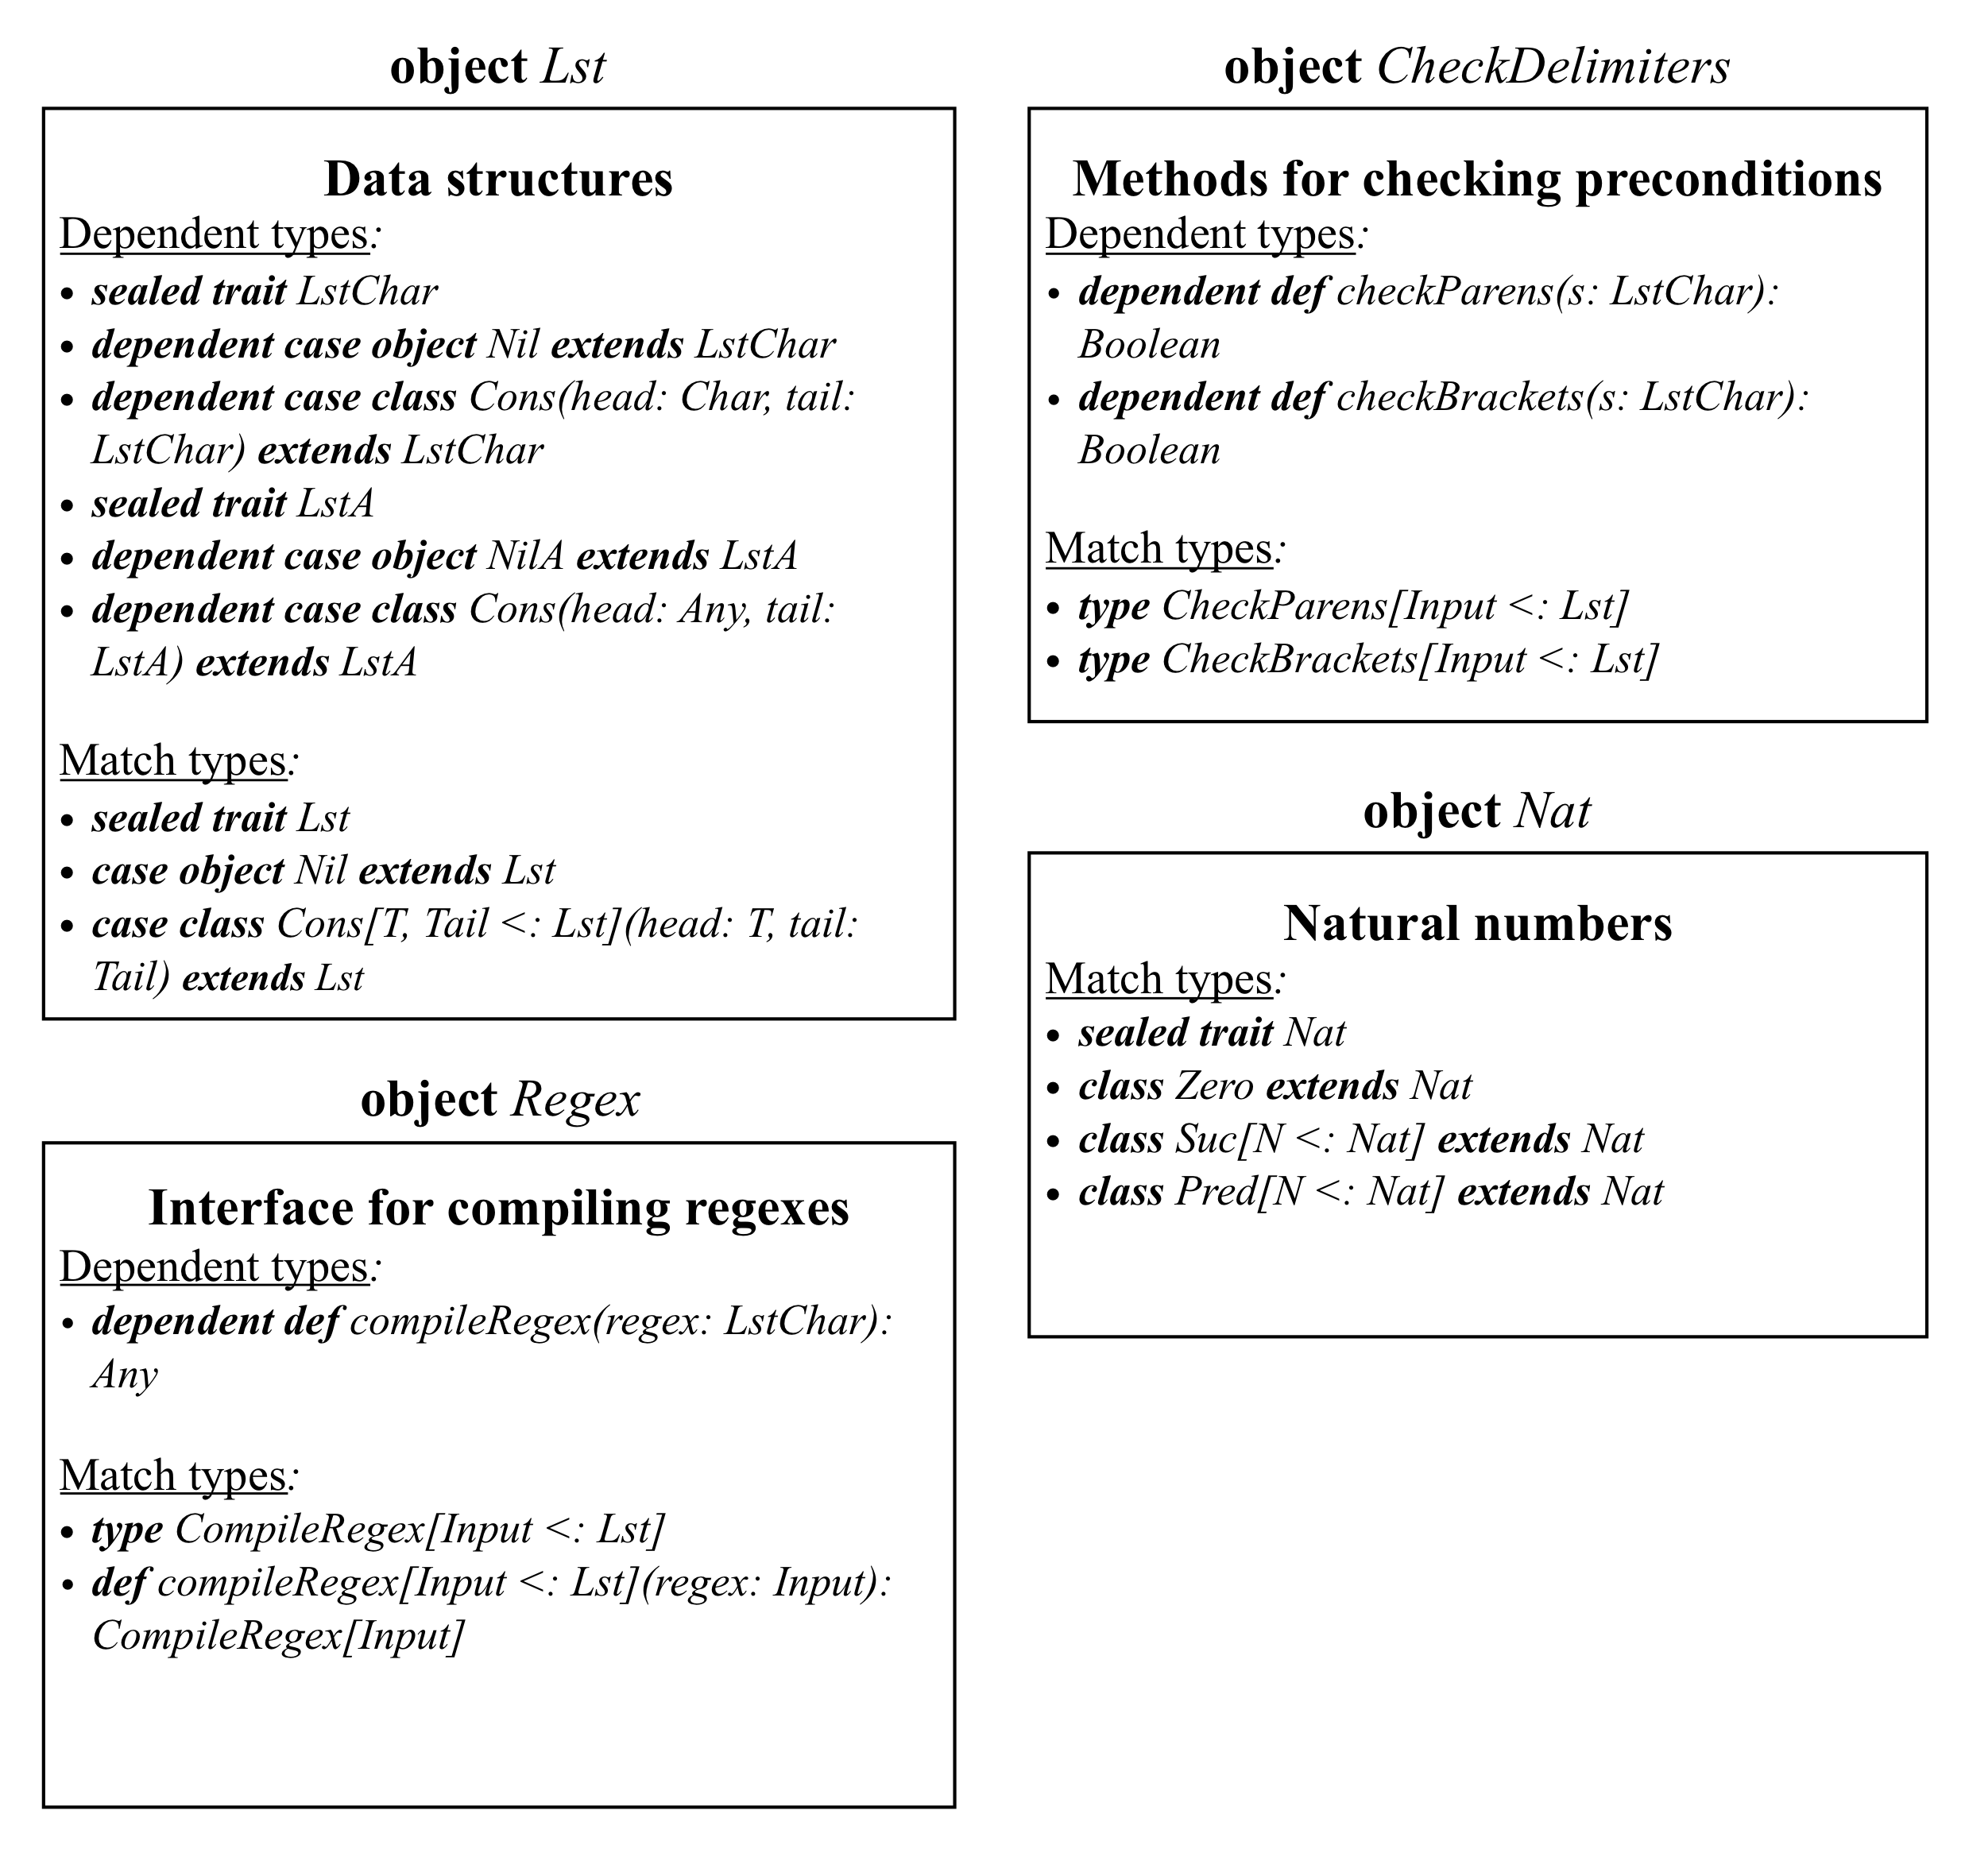
\includegraphics[scale=0.8]{images/structure.png}
\end{center}
\caption{The project structure described in Section \ref{architecture}.}
\label{structure.png}
\end{figure}

\twocolumn

\section{Implementation}\label{implementation}
In this section, we give an overview of how we used Dotty\textquotesingle s experimental functionalities, such as match types and dependent types, to improve the expressiveness of the Scala standard library for regular expressions.

First, we will describe the overall architecture of our extension and the approach taken for its implementation. Then, we will present, in more details, the core of our work that uses these new features, and the algorithm behind it.

\subsection{Architecture}\label{architecture}
We applied a functional approach to our work, relying on recursion and accumulators and avoiding side effects. Since the project main goal is to provide more insight into the use of dependent and match types, we decided to implement only a subset of regular expressions, focusing on readability rather than performance. For this reason, the supported functionalities are limited to capturing groups, simple character classes of the form [a-z], Kleene star * and optional ?.

The structure of the code, for both implementations, can be summarized into three modules (see Figure \ref{structure.png}): data structures for representing regexes, groups types and results (object \textit{Lst}), methods for checking preconditions and input format validity (object \textit{CheckDelimiters}) and the main interface used for compiling regular expressions (object \textit{Regex}). For the implementation involving match types, we have to add to this general structure also natural numbers (object \textit{Nat}), which are needed for type-level computations.

\subsection{Algorithm}
The bulk of the work is performed by a simple state machine, which consumes the regex one character at a time, iteratively building up the list containining the types corresponding to each group. This list and the Scala library for regular expressions are then used to construct a closure of the form \textit{String => Option[Cons(type, Cons(..., Nil)]}. This closure has complete knowledge of the regex groups\textquotesingle \space types at compile time and represents the pattern used to match the regex at run-time.
For example, compiling the regex "[a-z]" returns a closure of type \textit{String => Option[Cons(Char, Nil)]}.

\subsubsection{Dependent types}

\begin{lstlisting}[style=myScalastyle, caption={Dependent types prototypes.}, captionpos=b, label={dependent:code}]
dependent def compileRegex(regex: LstChar): Any = {
    if (checkParens(regex)) compile(regex, Empty, 0, false, 0, Nil, regex)
    else RegexError
}

dependent private def compile(..., groupsTypesRepr: LstChar, ...): Any = {... buildPattern(...) ... 
      ... compileCharClass(...) ...}

dependent private def compileCharClass(..., groupsTypesRepr: LstChar, ...): Any = {...}

dependent private def buildPattern(..., groupsTypesRepr: LstChar): String => Option[{ groupsTypesRepr.toLstA }] = { input: String => ...}.asInstanceOf[String => Option[{ groupsTypesRepr.toLstA }]]
\end{lstlisting}

In Listing \ref{dependent:code}, dependent types are used to keep the type of the list \textit{groupsTypesRepr} as precise as possible, in such a way that it can then be used as return type without information loss in the function \textit{buildPattern()}.

First, \textit{compileRegex()} checks that the regular expression is well formatted. Then, it calls \textit{compile()} which does most of the work; it keeps track of the type of the current group traversed (\textit{Empty}, \textit{Str}, \textit{Chr} or \textit{Integ}, defined as dependent case objects in object \textit{Regex}), the number of characters encountered (to distinguish between String and Char), whether a character class is present at the moment and how many are defined (to disambiguate between a group containing just a single char class, of type Char, and one containing multiple classes, of type String). The regex is cached as it is needed in \textit{buildPattern()}, where it is transformed in an actual scala.util.matching.Regex.

When a character class is encountered, \textit{compile()} checks that the brackets are balanced, and then relinquishes control to \textit{compileCharClass()}. This function parses the received regex, extracting the class type and eventually detecting errors (such as "[z-a]").

Finally, the function \textit{buildPattern} builds the closure to be used as pattern at run-time. Its body makes use of the Scala standard library to match the given input, and uses the information collected in \textit{groupsTypesRepr} to change the type of each group from the default one, String, to the actual, more informative type. 

\subsubsection{Match types}

\begin{lstlisting}[style=myScalastyle, caption={Match types prototypes.}, captionpos=b, label={match:code}]
type CompileRegex[Input <: Lst] = CheckParens[Input] match {
        case true => Compile[Input, Empty.type, Zero, false, Zero, Nil.type, Input]
        case false => RegexError.type
}

type Compile[..., GroupsTypesRepr <: Lst, ...] = ... match {
    ... BuildPattern[...] ... 
    ... CompileCharClass[...] ...
}

type CompileCharClass[..., GroupsTypesRepr <: Lst, ...] = ...

type BuildPattern[GroupsTypesRepr <: Lst] = String => Option[ToTypesList[GroupsTypesRepr]]
\end{lstlisting}

In Listing \ref{match:code}, match types are exploited in a similar way as dependent types. In fact, the actual implementation almost mirrors the dependent one, with the notable exception that actual Scala lists are used for the code executing at run-time (functions \textit{compile()}, \textit{compileCharClass()} and \textit{buildPattern()}). For this reason, we decided to highlight in this section only the type-level implementation, as it shows how match types can be used to achieve the same purpose as dependent ones with the same algorithm and few syntax changes.

The types thus defined are used as return types for the functions of the same name (Figure \ref{structure.png} shows an example).


\section{Use cases}
In this section, we present two concrete examples that demonstrate the advantages of using strongly-typed, expressive regular expressions over the weakly-typed, string-based ones implemented in the Scala standard library.

The examples highlight the benefits of knowing precisely the types of the capturing groups at compile time and show how it is possible to use this additional information to increase type-safety and reliability.

\subsection{Matching URLs}

In this use case, we first create a regular expression for matching URLs. Then, we extract the information retrieved from a match, storing it in a case class \textit{URL()}. Finally, we perform an operation on one of the fields, protocol.

\subsubsection{Scala regular expressions}

As illustrated in Listing \ref{URL:scala}, in the Scala standard library, if an optional expression (resulting from a *, for instance) is not present, its value will be null upon matching. Thus, assuming that it has been decided beforehand that null values will be treated as \textit{None}, the programmer has to explicitly handle this case, through cumbersome if-conditions or using the \textit{Option()} constructor. On the other hand, if the user, by accident, forgets to perform these checks, the program will fail with an exception at run-time. 

\subsubsection{Regular expressions with dependent and match types}

With dependent and match types (Listing \ref{URL:match}), however, if an optional expression is not present, its value is \textit{None} by default and its actual type is known at compile time. This means that the programmer does not have to perform null checks, because he is protected by the compiler\textquotesingle s type-checker. The resulting code is thus easier to write and safer to use, because errors will be caught early, at compile time.

\subsection{Matching sbt compilation results}
In this second example, we create a regular expression for matching sbt compilation results, and use it to extract the total compilation time.

The code is available in Listings \ref{sbt:scala} and \ref{sbt:dependent}.

\onecolumn

\begin{lstlisting}[style=myScalastyle, caption={Matching URLs with Scala regex.}, captionpos=b, label={URL:scala}, basicstyle={\small\ttfamily}]
case class URL(protocol: Option[String], hostname: String, domain: String, path: Option[String])

val regexURL: Regex = "(https?://)?(www.)?([a-z][a-z]*)(.)([a-z][a-z][a-z]*)(/[a-z]*)*".r
val url: Option[URL] = "https://www.epfl.ch/schools/ic/" match {
    // if an optional is not present, its value is null
    case regexURL(protocol, _, hostname, _, domain, path) => 
        // since the Regex extractor produces varargs, the user could use the wrong group
        Some(URL(Option(protocol), hostname, domain, Option(path))) 
    case _ => None
}
// if the user forgets to do null checks, this call fails with an exception at run-time
val protocolName: String = extractProtocolName(url) 
\end{lstlisting}

\begin{lstlisting}[style=myScalastyle, caption={Matching URLs with match types.}, captionpos=b, label={URL:match}]
case class URL(protocol: Option[String], hostname: String, domain: String, path: Option[StarMatch[String]])

val regexURL: String => Option[Cons[Option[String], Cons[Option[String], Cons[String, Cons[Char, Cons[String, Cons[Option[StarMatch[String]], Nil.type]]]]]]] = compileRegex[...](...)
val url: Option[URL] = regexURL("https://www.epfl.ch/schools/ic/") map {
        // if an optional is not present, its value is None and its type is known at compile time
        case Cons(protocol, Cons(_, Cons(hostname, Cons(_, Cons(domain, Cons(path, _)))))) => URL(protocol, hostname, domain, path)
}
val protocolName: String = extractProtocolName(url) 
\end{lstlisting}

\begin{lstlisting}[style=myScalastyle, caption={Matching sbt compilation results with Scala regex.}, captionpos=b, label={sbt:scala}]
val regexCompilationResult: Regex = "(Total time: )([0-9][0-9]*)( s, completed )([A-Z][a-z]*)( )([0-9][0-9]?)(, )([0-9][0-9][0-9][0-9])( )([0-9][0-9]?)(:)([0-9][0-9])(:)([0-9][0-9])( )([A-Z][A-Z])".r
val compilationTime: Option[Int] = "Total time: 228 s, completed May 9, 2019 7:33:37 PM" match {
    // if we call toInt on the wrong group, we get an exception at run-time
    case regexCompilationResult(_, time, _: _*) => Some(time.toInt)
    case _ => None
}
\end{lstlisting}

\begin{lstlisting}[style=myScalastyle, caption={Matching sbt compilation results with dependent types.}, captionpos=b, label={sbt:dependent}]
val regexCompilationResult: String => Option[{ ConsA(_ : String, ConsA(_ : Int, ConsA(_ : String, ConsA(_ : String, ConsA(_ : Char, ConsA(_ : Int, ConsA(_ : String, ConsA(_ : Int, ConsA(_ : Char, ConsA(_ : Int, ConsA(_ : Char, ConsA(_ : Int, ConsA(_ : Char, ConsA(_ : Int, ConsA(_ : Char, ConsA(_ : String, NilA)))))))))))))))) }] = compileRegex(...)
val compilationTime: Option[Int] = regexCompilationResult("Total time: 228 s, completed May 9, 2019 7:33:37 PM") map {
    case ConsA(_, ConsA(time, _)) => time // completely safe
}
\end{lstlisting}

\twocolumn

\subsubsection{Scala regular expressions}

The standard library is, as stated before, weakly-typed: all values resulting from a match are represented as strings. Thus, in order to retrieve the compilation time as Int in Listing \ref{sbt:scala}, we have to call \textit{toInt()} on the expression corresponding to it. This operation is unsafe, because the programmer could use, for example, the wrong extracted group, which would lead to a run-time exception.

\subsubsection{Regular expressions with dependent and match types}

With our approach, there is no need to use \textit{toInt()}, because actual groups  types are computed at compile time. Hence, even if the user makes a mistake and extracts the wrong expression, the compiler will complain and catch the error.

\section{Results}
In this section, we compare the two methods presented in Section \ref{implementation}, using them as a basis for a more general analysis of Dotty\textquotesingle s current implementation of match and dependent types.

We start by analyzing their compilation time. Then, we briefly describe our experience in developing with them. Finally, we highlight some key differences we identified.

\subsection{Compile time comparison}

Benchmarks suggest that, in both implementations, the additional compilation time spent doing actual type-level computation is negligible compared to the overall compilation time. Moreover, compared to the Scala standard library, our work requires slightly more time to compile.

\subsection{Programming experience and ease of use}
Both features, for several reasons, are challenging to use. There is a general lack of documentation and of meaningful error messages, that, combined with sporadic bugs, makes programming with them more difficult. However, we found that slightly changing our programming habits to use them was the hardest part; sometimes, it was difficult to even understand how to approach a certain problem. This was especially true for match types, because pattern matching was the only language construct at disposal for pure type-level programming.

\subsubsection{Dependent types}

Programming with dependent types, even though pattern matching is not supported, is in general more similar to usual programming and thus easier. Nevertheless, it requires dependently-typed data structures and functions, which means that the standard library cannot be used. Hence, the programmer has to write everything on his own, from scratch. 

Since equality between objects is not yet understood by dependent types, we had to use Char to represent types. We were constrained in our implementation decisions also in other situations: closures defined in a dependent context do not work well (our usage of \textit{zipWithIndex()}, in the function \textit{BuildPattern()}, is an evidence) and types are not correctly inferred at run-time for the expression resulting from a regex pattern matching, and thus casts are necessary.

\subsubsection{Match types}

Match types are arguably harder to code with, since they compel the user to program at the type level. The resulting programs are, however, easier to read and more elegant, despite being more verbose. Their elegance, compared to the dependently-typed ones, can be appreciated because the Scala standard library and pattern matching are available for usage. 

Duplicated code is the main problem with match types. The code written for a function and the corresponding type-level code are essentially the same (\textit{Compile[]} and \textit{compile()} are clear proof). Furthermore, upon function calls, as it is done for polymorphic methods, all types must be specified (including potentially long type-level regexes in our implementation) which can be tedious, error-prone and another source of code duplication.

Another limitation we encountered is the impossibility to perform inequality comparisons on types. This prevents error detection in character classes when the first element is greater than the second.

Finally, it is not possible to perform arithmetic operations or simple counting on integers at the type level, which led us to use type-level natural numbers instead.

\section{Conclusion}
In this report, Dotty\textquotesingle s dependent types and match types have been proved capable of trading off compile time performance and ease of use for additional type safety. Here, some possible extensions and improvements to the presented regex library are described.

The current work covers a subset of regular expressions; a natural extension would be to support a larger subset, such as +, \^{} (not) or even | (or), although at the moment match and dependent types do not allow it. It would also be useful to have predefined character classes, such as \textbackslash{}d for a digit, and more advanced ones, such as [a-zA-Z]. Quantifiers of the form X\{n\} (X exactly n times) would be also relatively easy to implement. A major addition would be allowing nested capturing groups, but they would be more complicated to provide without significant changes to the algorithm.

\bibliographystyle{abbrv}
\bibliography{bibliography.bib}

\end{document}
